\documentclass[tikz,border=6pt]{standalone}
\usepackage[T1]{fontenc}
\usepackage[utf8]{inputenc}
\usepackage{pgfplots}
\usepgfplotslibrary{groupplots}
\usetikzlibrary{calc}
\pgfplotsset{compat=1.18}
\begin{document}
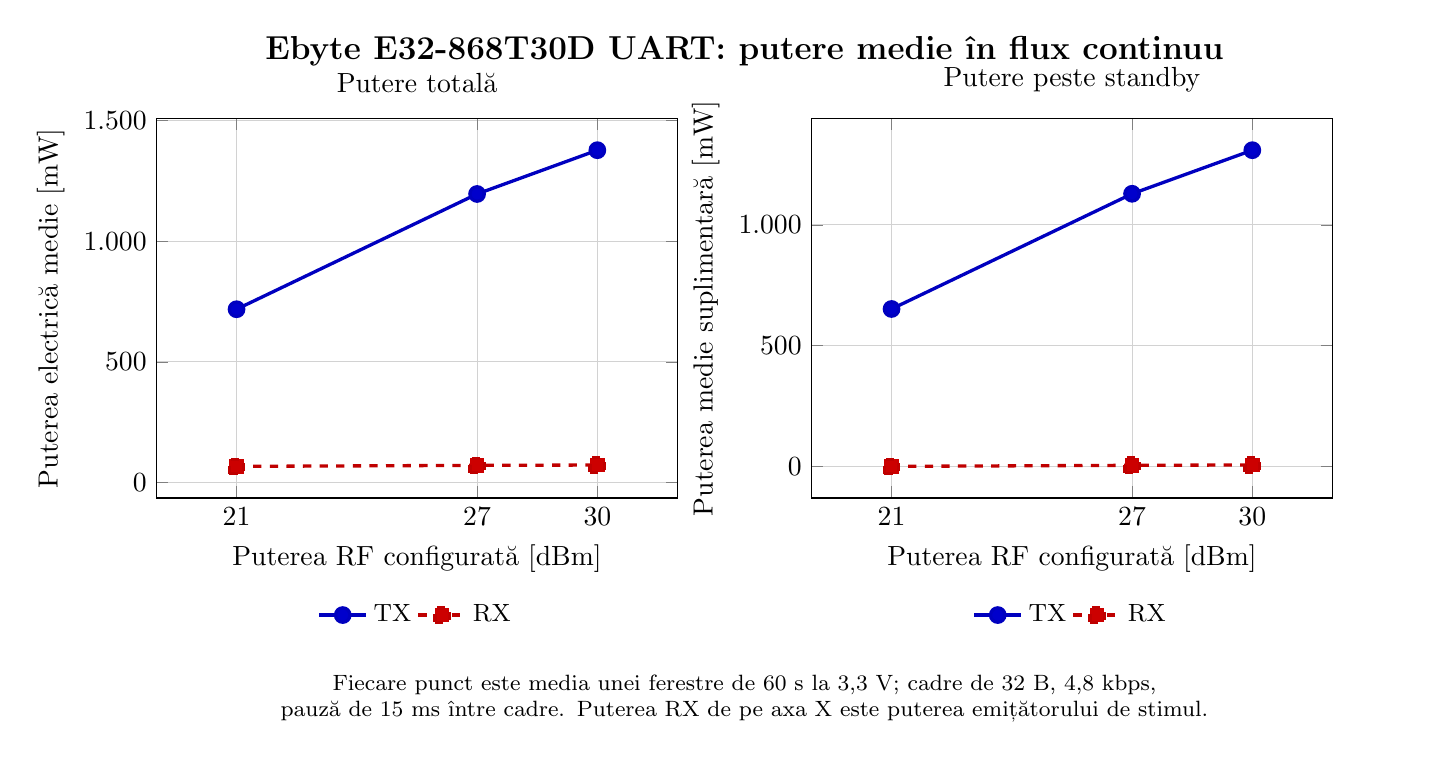
\begin{tikzpicture}
\begin{groupplot}[/pgf/number format/use comma,
  group style={group size=2 by 1, horizontal sep=1.7cm},
  width=8.2cm, height=6.4cm,
  xmin=19, xmax=32, xtick={21,27,30},
  xlabel={Puterea RF configurată [dBm]},
  grid=both, minor grid style={gray!15}, major grid style={gray!35},
  every axis plot/.append style={line width=1.2pt, mark size=2.6pt},
  legend style={font=\small, draw=none, fill=none,
    at={(0.5,-0.25)}, anchor=north, legend columns=2},
]
\nextgroupplot[title={Putere totală}, ylabel={Puterea electrică medie [mW]}]
\addplot+[blue!75!black, mark=*] coordinates {(21,717.767004) (27,1195.51178) (30,1376.96612)};
\addlegendentry{TX}
\addplot+[red!75!black, dashed, mark=square*] coordinates {(21,66.5095299) (27,70.6846451) (30,72.1219219)};
\addlegendentry{RX}
\nextgroupplot[title={Putere peste standby}, ylabel={Puterea medie suplimentară [mW]}]
\addplot+[blue!75!black, mark=*] coordinates {(21,651.685105) (27,1128.67106) (30,1309.1206)};
\addlegendentry{TX}
\addplot+[red!75!black, dashed, mark=square*] coordinates {(21,0) (27,4.31788543) (30,5.87814862)};
\addlegendentry{RX}
\end{groupplot}
\node[font=\bfseries\large] at ($(group c1r1.north)!0.5!(group c2r1.north)+(0,0.85cm)$)
  {Ebyte E32-868T30D UART: putere medie în flux continuu};
\node[font=\footnotesize, align=center, text width=16.5cm]
  at ($(group c1r1.south)!0.5!(group c2r1.south)+(0,-2.55cm)$)
  {Fiecare punct este media unei ferestre de 60 s la 3,3 V; cadre de 32 B, 4{,}8 kbps,\\
   pauză de 15 ms între cadre. Puterea RX de pe axa X este puterea emițătorului de stimul.};
\end{tikzpicture}
\end{document}
